\label{sec:results}
\section{Results}

\subsection{Criticalities}

One of the main goals of the project was to test the feasibility of a room-sized reactor for research purposes. The room-size aspect is key here for initial criticality calculations. The shell radius was first taken to be $r=10cm$, resulting in a reactor just over 20cm on its length, width and height. However, the core was not critical enough at these dimensions, and hence the radius was increased to $r=100cm$. This was done in order to accommodate a larger core to get a k-coefficient of $k=1$.

The first step was to determine the relationship between the size of the core (in these simulations, pure U-235), and the criticality. From table \ref{tab:pure}, the relationship is seen to be linear.

\begin{table}[!htbp]
\centering
\caption{Pure U-235 core in water without shell}
\label{tab:pure}
\begin{tabular}{|c|c|c|c|c|}
\hline
Composition & Side length (cm) & Shell material & Submergence & k-coefficient \\
\hline
Pure U-235  & 10               & N/A            & Water       & 1.26          \\
\hline
Pure U-235  & 20               & N/A            & Water       & 1.49408       \\
\hline
Pure U-235  & 30               & N/A            & Water       & 1.76348       \\
\hline
\end{tabular}
\end{table}

The linear relationship applies holds in the case when the core is in vacuum. An important note here is the fact that particles were not bounced back into the core - they disappeared at the graveyard boundary. The k-coefficients are less here due to the surrounding empty space - table \ref{tab:purevac}.

\begin{table}[!htbp]
\centering
\caption{Pure U-235 core in vacuum without shell}
\label{tab:purevac}
\begin{tabular}{|c|c|c|c|c|}
\hline
Composition & Side length (cm) & Shell material & Submergence & k-coefficient \\
\hline
Pure U-235  & 10               & N/A            & Vacuum       & 0.74311      \\
\hline
Pure U-235  & 20               & N/A            & Vacuum       & 1.30614       \\
\hline
Pure U-235  & 30               & N/A            & Vacuum       & 1.64085       \\
\hline
\end{tabular}
\end{table}

Knowing the results without a shell, a zirconium enclosing was added to reflect the neutrons back into the core to trigger further reactions. Looking at the values in tables \ref{tab:purezrv} and \ref{tab:purezrw}, the zirconium did not have any significant effect on the k-coefficients with the larger core. This does make sense since the metal allows neutrons to travel freely through it. However, for the first variation, the coefficient decreased from 1.26 to 0.99284. This is assumed to be a sampling error due to the number of cycles used.

\begin{table}[!htbp]
\centering
\caption{Pure U-235 core in water with zirconium shell}
\label{tab:purezrw}
\begin{tabular}{|c|c|c|c|c|}
\hline
Composition & Side length (cm) & Shell material & Submergence & k-coefficient \\
\hline
Pure U-235  & 10               & Zirconium            & Water       & 0.99284      \\
\hline
Pure U-235  & 20               & Zirconium            & Water       & 1.49408       \\
\hline
Pure U-235  & 30               & Zirconium            & Water       & 1.76348       \\
\hline
\end{tabular}
\end{table}

\begin{table}[!htbp]
\centering
\caption{Pure U-235 core in vacuum with zirconium shell}
\label{tab:purezrv}
\begin{tabular}{|c|c|c|c|c|}
\hline
Composition & Side length (cm) & Shell material & Submergence & k-coefficient \\
\hline
Pure U-235  & 10               & Zirconium            & Vacuum       & 0.74275      \\
\hline
Pure U-235  & 20               & Zirconium            & Vacuum       & 1.30478       \\
\hline
Pure U-235  & 30               & Zirconium            & Vacuum       & 1.64499       \\
\hline
\end{tabular}
\end{table}

Generally, the zirconium shell had a negative impact on the criticality of the core. This is evidenced by the slightly increased k-coefficients seen in table \ref{tab:puregraphite}, where a graphite shell was used instead\footnote{Interestingly enough, MCNP was unable to normalize particle scattering for these simulations. As a result, the number of k-cycles, or samples, was doubled from 115 to 230 for these runs.}.

\begin{table}[!htbp]
\centering
\caption{Pure U-235 core in vacuum with graphite shell}
\label{tab:puregraphite}
\begin{tabular}{|c|c|c|c|c|}
\hline
Composition & Side length (cm) & Shell material & Submergence & k-coefficient \\
\hline
Pure U-235  & 10               & Graphite            & Vacuum       & 0.74659      \\
\hline
Pure U-235  & 20               & Graphite            & Vacuum       & 1.30598       \\
\hline
Pure U-235  & 30               & Graphite            & Vacuum       & 1.64367       \\
\hline
\end{tabular}
\end{table}

The results are even better with water acting as the moderator, as seen in table \ref{tab:puregraphitew}.

\begin{table}[!htbp]
\centering
\caption{Pure U-235 core in water with graphite shell}
\label{tab:puregraphitew}
\begin{tabular}{|c|c|c|c|c|}
\hline
Composition & Side length (cm) & Shell material & Submergence & k-coefficient \\
\hline
Pure U-235  & 10               & Graphite            & Water       & 1.21312      \\
\hline
Pure U-235  & 20               & Graphite            & Water       & 1.57019       \\
\hline
Pure U-235  & 30               & Graphite            & Water       & 1.78865       \\
\hline
\end{tabular}
\end{table}

From the above tables, one can see that the optimum combination is to have the core submerged in water, with a graphite shell reflecting the neutrons back into the system. The issue with the above simulations is that the core is made up of pure U-235, which is weapons grade. Table \ref{tab:variations} shows tested combinations of size and enrichment levels to achieve the optimum k-coefficient of $k=1$.

\begin{table}[!htbp]
\centering
\caption{Core size and enrichment variations}
\label{tab:variations}
\begin{tabular}{|c|c|c|}
\hline
Composition            & Side length (cm) & k-coefficient \\
\hline
U-238, 20\% enrichment & 10               & 0.85447       \\
\hline
U-238, 20\% enrichment & 20               & 1.02792       \\
\hline
U-238, 20\% enrichment & 30               & 1.15384       \\
\hline
U-238, 20\% enrichment & 60               & 1.40225       \\
\hline
U-238, 15\% enrichment & 60               & 1.27469       \\
\hline
U-238, 15\% enrichment & 40               & 1.15583       \\
\hline
U-238, 15\% enrichment & 30               & 1.06625      \\
\hline
\end{tabular}
\end{table}

To finalize the initial geometries, one more variable was looked at - the radius of the shell. In all simulations, this value did not affect the criticality, so the radius was decreased to $r=50cm$, which created for a more compact reactor chamber to work with. Since the radius has no effect on the criticality, the shell can be adjusted at will to reflect the neutrons more efficiently back into the core.

\subsection{Reactor designs}
Through the criticality results, the first design of the reactor is seen below, in figure \ref{fig:design1}. The improved, geometrically optimized reactor design is seen below that, in figure \ref{fig:design2}.
\begin{figure}[!htbp]
\caption{First reactor design.}
\label{fig:design1}
\centering
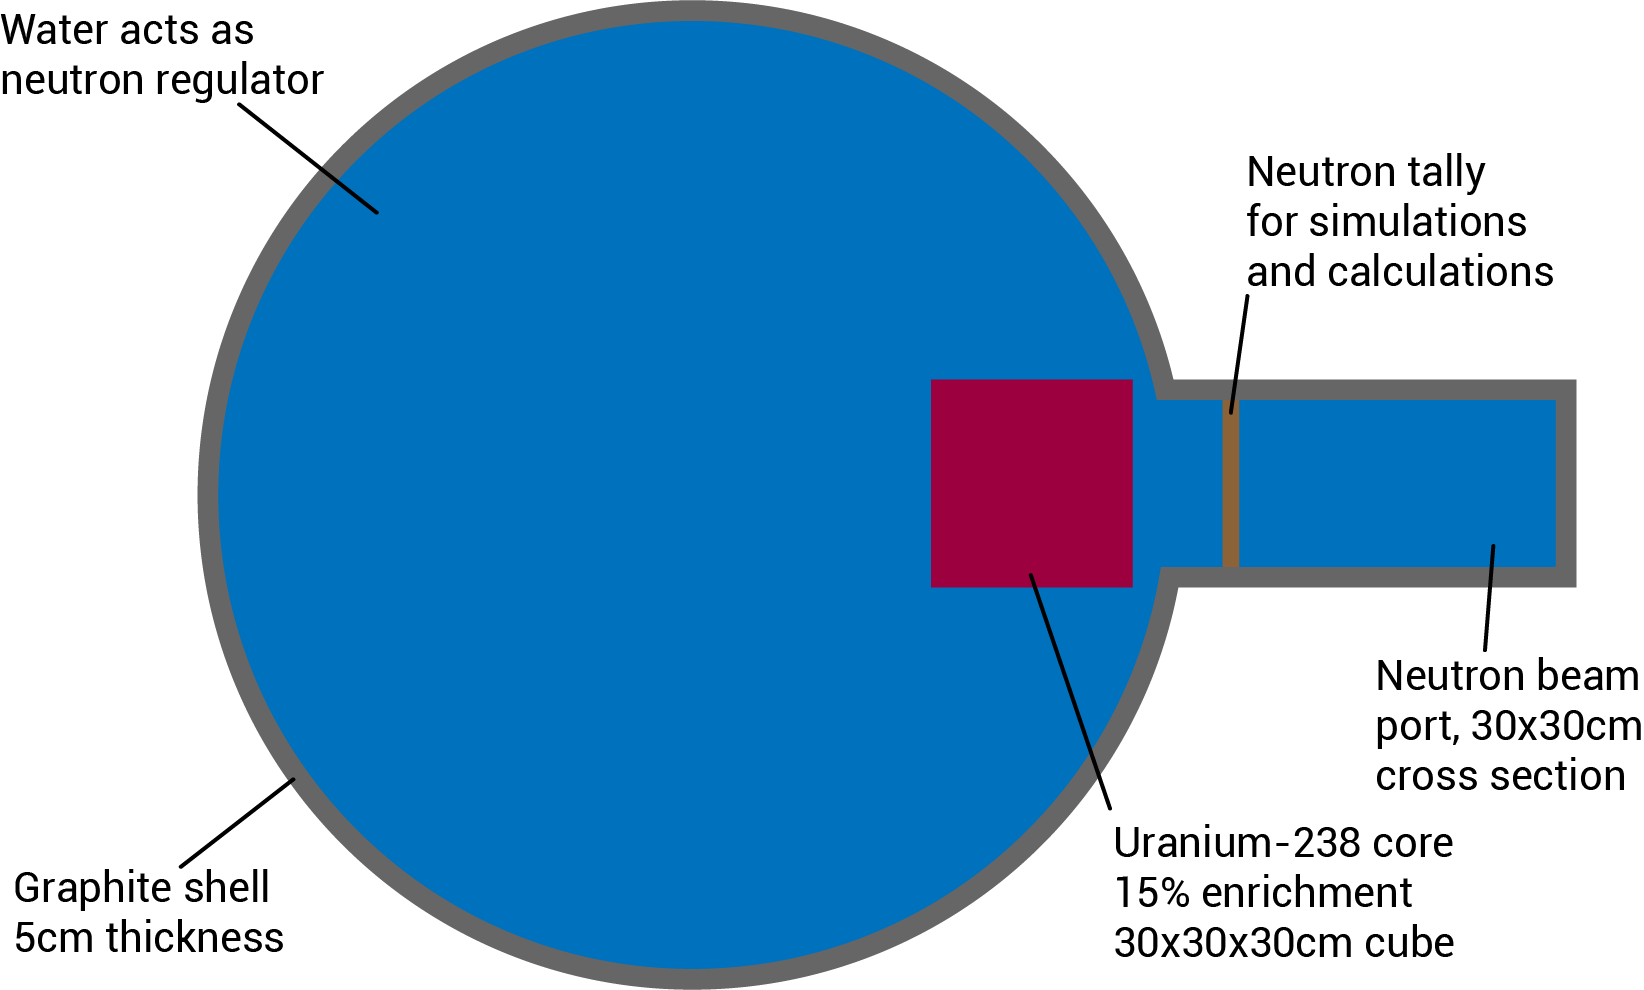
\includegraphics[width=0.75\textwidth]{design.png}
\end{figure}

\begin{figure}[!htbp]
\caption{Improved reactor design.}
\label{fig:design2}
\centering
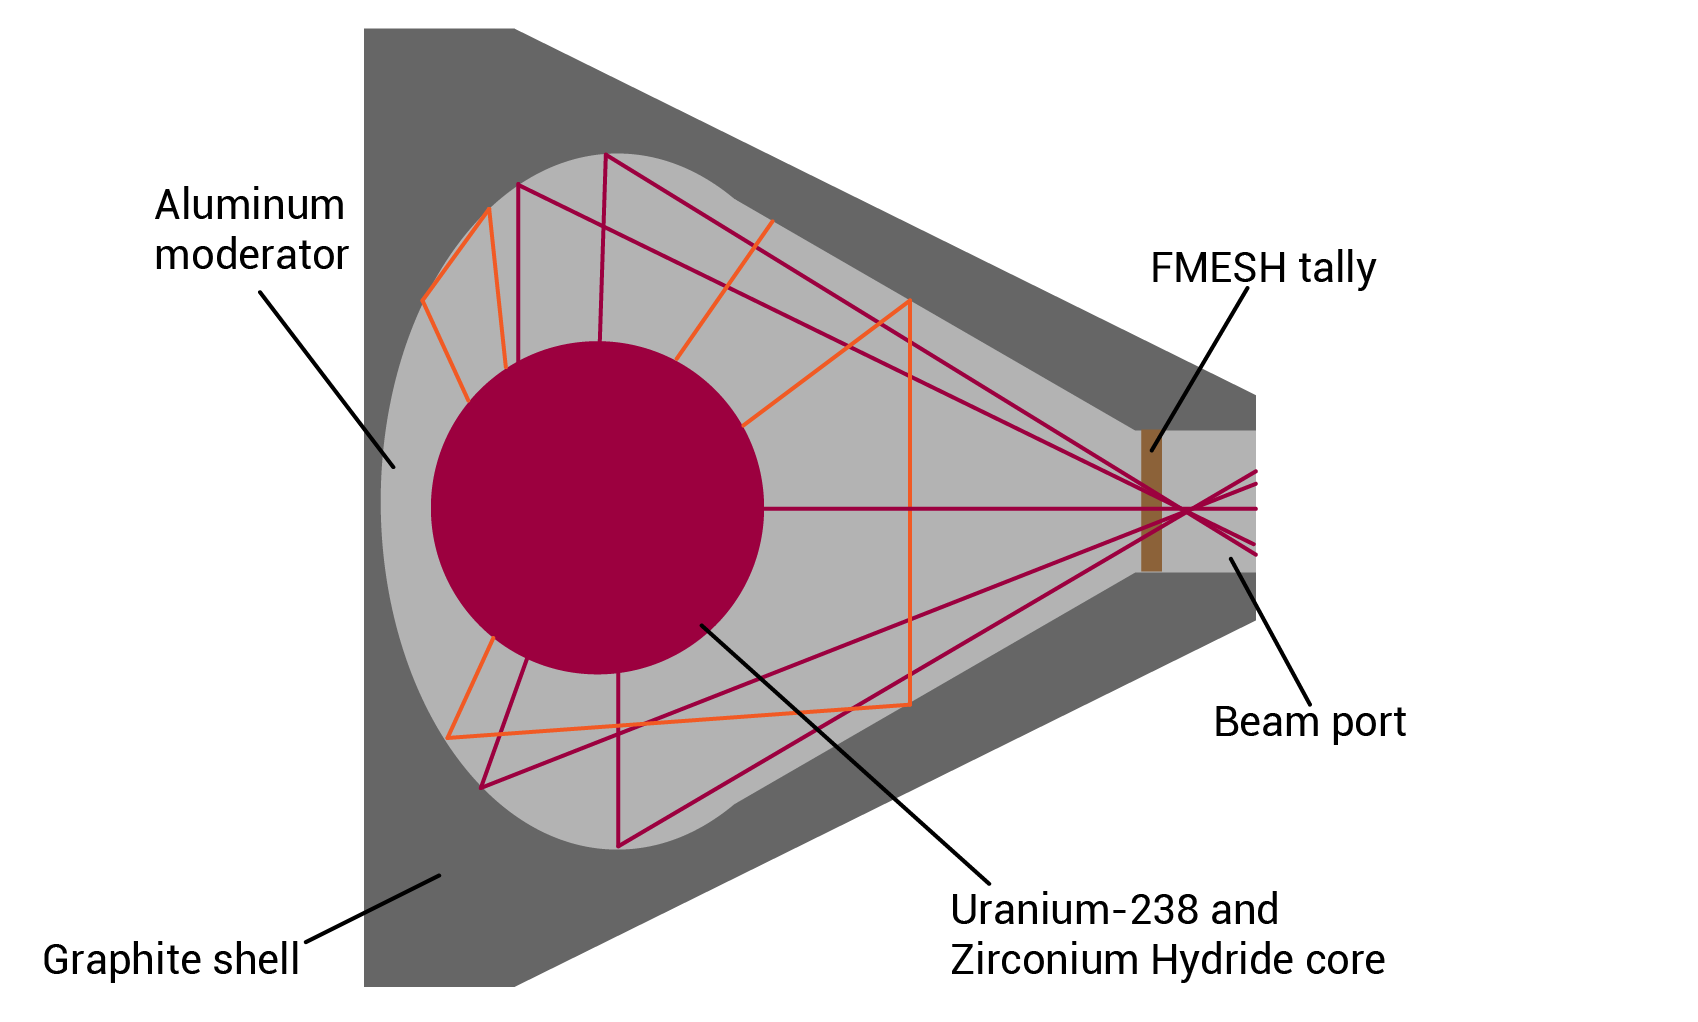
\includegraphics[width=0.85\textwidth]{design2.png}
\end{figure}
\subsection{Tallies}
%Need math confirmation to finish this bit....